\documentclass[a4paper,11pt]{article}

\usepackage{float}
\usepackage{graphicx}
\graphicspath{./Diagrams}

\setlength{\oddsidemargin}{0in}
\setlength{\evensidemargin}{0in}
\setlength{\textwidth}{160mm}
\setlength{\topmargin}{-15mm}
\setlength{\textheight}{240mm}


\begin{document}
\section{Background}

\subsection{Problem description}
The logic based combinatorial number placement puzzle Sudoku, is a well-established puzzle game which grew popular in Japan in the 1980s. The classic game of Sudoku consists of a 9x9 grid of spaces, which can only be filled with numbers between 1 and 9. Each space in the 3x3 block, vertical and horizontal columns can only have each number between 1 and 9 once. The puzzle is completed when all spaces in the grid have been filled and no earlier rule has been violated. A more generic description of the puzzle, describes a grid of NxN in size, with N grids contained, using numbers between 1-N. []
\begin{figure}[h]
	\caption{Example Sudoku puzzle(left), Examples of different violations(right)}
	\centering
	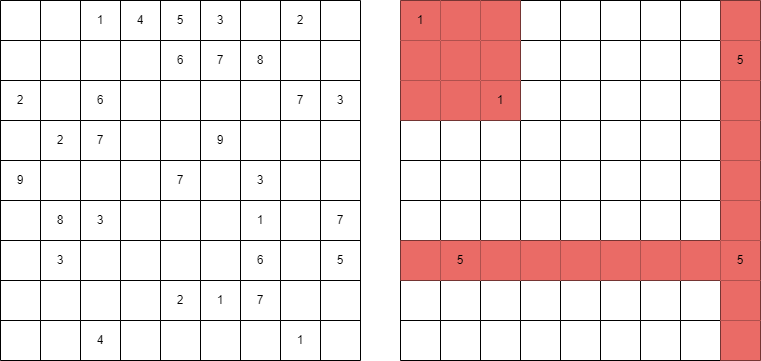
\includegraphics[height=5cm, width=10cm]{./Diagrams/violationExample}
\end{figure}

\subsection{Background}
Sudoku is a well established and solved puzzle, with a proven efficient way to be solved established. However, there are other admittedly less efficient AI methods which can be applied to solve this and provides an interesting way to apply and experiment with AI methods learnt at university to a real problem.\newline \newline
Peter Norvig solved Sudoku [], using both constraint propagation and search, so the most efficient method is too established. However, looking at a book[], using a different heuristic search approach seems to be a better way, which has been used before but not fully explored was in there. \newline \newline
Using evolutionary algorithms(EA), specifically based off the Russel/Norvig approach [] to solve seems like an interesting and most importantly different way to solve the problem, which can also solve several different size puzzles with some level of efficiency. Equally a normal evolutionary algorithm on its own will need some help to be able to solve the sudoku at all leaving several different options, this includes using different hybrid methods to add constraints to the problem, or having constraints included as part of the evolutionary algorithms fitness function.\newline\newline
EA has several terms that will be used throughout this report.\\
\begin{itemize}
	\item Population - The total number of individuals in the algorithm
	\item Individual - Each state used to represent the objects the algorithm is solving
	\item Fitness function - A function used to rate each individual in the population based on viable a solution it is
	\item Selection - The process of taking only a section of the population based on their fitness
	\item Crossover - The process of mixing parts of the individuals to produce new variation children 
	\item Mutation -  The process of randomly changing a gene within individuals
	\item Multi-objective EA - Where the fitness function uses more than one numerical value to rate each individual
\end{itemize}
\subsection{Analysis}
The evolutionary algorithm will need a few key items at implementation:
\begin{itemize}
	\item A way to encode the puzzle
	\item A fitness function
	\item A selection process for the population
	\item A mutation function
\end{itemize}
For the fitness function there are two different ways it can be done, a simple fitness function which does not enforce the rules of sudoku, this would need a hybrid approach to help enforce the rules. Alternatively, a more complex fitness function, that considers several factors, to look at fitness i.e., a multi-objective evolutionary algorithm.\newline \newline
For solving the sudoku a hybrid evolutionary algorithm, there are several different hybrid approaches existing []. The recommended approach for a constraint optimization problem such as sudoku is a repair method. The repair method would work to enforce the rules of the puzzle, by changing each individual in the population that violates the constraints bringing it back into the range of viable solutions.\newline \newline
These two different methods both have valid ways of solving the Sudoku and create a new question. Does a hybrid approach using a repair method work better than a classical approach using multi-objective EAs? They can be compared on, number of generations, runtime, number of puzzles stuck on and looks at patterns between different sudoku puzzle difficulties and seeing if the pattern of human difficulty has any relationship to how long it takes for each EA to solve the puzzle.

\subsection{Process}
The lifecycle model used in this project, takes the most helpful aspects of different life-cycles, and applies them to be of the most use in this project. The most important and closely followed part of the process is the use of the Kanban board, used to keep track of what tasks there were to do. From Scrum the ideas of sprints and stories are used to build up a log of tasks which are used on the Kanban board and a weekly meeting which were used to review what work had been done that week, discuss improvements on that work and talk about targets for the next week.\newline \newline However, the underlying process used in project is closer to waterfall, with the requirements and research being done first, followed up by implementation, testing and maintenance. Overall, it would describe the process as waterfall with different agile aspects.

\end{document}